%\documentclass[12pt,fleqn, leqno, acm]{article}
\documentclass[12pt]{article}

%% Estilos e Plug-Ins
%\usepackage{a4wide}
\usepackage{a4}
\ifx\pdfoutput\undefined
   \usepackage[dvips]{graphicx}
\else
   \usepackage[pdftex]{graphicx}
\fi
\usepackage{times}
\usepackage{isolatin1}
\usepackage[brazil]{babel}
\usepackage{fancyheadings}
\usepackage{lastpage} 

\pagestyle{fancy}

\textheight=8.2in
%\headwidth=1.2\textwidth
\lhead{\setlength{\unitlength}{1mm} 
\begin{picture}(0,0) 
\put(5,0){\includegraphics[width=0.8in]{figs/fundacao.pdf}} 
\end{picture}} 
\chead{}
\rhead{\setlength{\unitlength}{1mm} 
\begin{picture}(0,0) 
\put(5,0){\includegraphics[width=0.8in]{figs/tecgraf.pdf}} 
\end{picture}} 

\lfoot{\scriptsize %
Tecgraf/PUC-Rio \hfill -
\hfill Rua Marqu�s de S�o Vicente, 225 - Pr�dio Velloso \hfill -
\hfill CEP 22453-900 \hfill - \hfill Rio de Janeiro -- Brasil\\
Tel. +55 21 512-5984 - Fax. +55 21 259-2232 \hfill -
\hfill E-mail: openbus@tecgraf.puc-rio.br \hfill -
\hfill URL: http://www.tecgraf.puc-rio.br\\
\vspace{0.5cm} 
\today \hfill P�gina \thepage \hspace{0.1cm} de \pageref{LastPage}} 
%27/6/2006	P�ina 1 de 33
\cfoot{}
\rfoot{}

\addtolength{\parskip}{\baselineskip}

%\hyphenation{
%in-te-gra-\c{c}\~oes
%apli-ca-\c{c}\~oes
%}

% ===================
% In�io do documento
% ===================
\begin{document}

\title{OpenBus}
\author{}
\date{}
\maketitle
\thispagestyle{empty}

\section{Introdu��o}
\label{introducao}

A unidade de Explora��o e Produ��o (E\&P) da Petrobras possui diversas
aplica��es que s�o utilizadas por seus funcion�rios na realiza��o dos seus
fluxos de trabalho. Existem aplica��es desenvolvidas pela pr�pria Petrobras,
desenvolvidas em parceria com universidades ou compradas de terceiros.
Embora essas aplica��es trabalhem bem individualmente, o fluxo de trabalho de
um funcion�rio pode envolver a utiliza��o de mais de uma dessas aplica��es
e, como essas aplica��es foram desenvolvidas para serem executadas de maneira
independente, qualquer troca de dados deve ser realizada manualmente pelos
funcion�rios (os usu�rios das aplica��es).

Para diminuir a participa��o manual do usu�rio no papel de integrador, algumas
aplica��es j� est�o oferencendo mecanismos para que outras aplica��es acessem
seus dados. Como exemplo temos o WebSintesi e o Sigeo que permitem acesso �s
suas �reas de projeto. O WebSintesi disponibiliza uma biblioteca para acesso �
sua �rea de projetos enquanto que o Sigeo possui um servidor que possibilita �s
aplica��es gravarem dados em sua �rea de projetos.

Algumas aplica��es especiais, os chamados sistemas integradores, v�m sendo
utilizados para facilitar a integra��o de aplica��es. Esses sistemas prov�em
uma infraestrutura b�sica para a cria��o de aplica��es que devem estar
integradas. O WebSintesi, por exemplo, realiza a integra��o de aplica��es de
an�lise e s�ntese de dados geof�sicos. Outro sistema integrador importante � o
OpenSpirit que integra e padroniza o acesso a dados de Geologia e Geof�sica
independente da forma como esses dados est�o armazenados nas suas
aplica��es originais. At� mesmo esses sistemas integradores est�o
integrados. O WebSintesi, por exemplo, acessa os dados disponibilizados
pelo OpenSpirit.

Nesse contexto, podemos apontar algumas dificuldades:

\begin{itemize}
\item {\bf O usu�rio ainda assume o papel de integrador entre v�rias aplica��es.}

O usu�rio precisa conhecer funcionalidades de aplica��es que
nem precisaria utilizar. O usu�rio do Sigeo, por exemplo, precisa saber
que a aplica��o VGE acessa os dados da base da s�smica e se quiser algum dado
contido nessa base - fei��es, por exemplo - ter� de usar o VGE para obt�-lo
para o seu projeto no Sigeo.

\item {\bf Dificuldade em integrar aplica��es Petrobras.}

O maior problema dsse tipo de integra��o pontual � que o n�mero de integra��es
tende a se tornar exponencial (\(\frac{n(n-1)}{2}\)). Se quis�ssemos integrar
10 aplica��es, dever�amos implementar 45 integra��es.

A integra��o de aplica��es Petrobras � bastante complexa, especialmente quando
as aplica��es s�o desenvolvidas por equipes diferentes. Para implementar
essas integra��es s�o adotadas solu��es espec�ficas para resolver o
problema. Nem sempre essa solu��o espec�fica pode ser reutilizada quando
uma integra��o similar � necess�ria. Seguem dois exemplos de
implementa��o atuais:
\begin{enumerate}
\item A integra��o do WebSintesi com o V3O2 � implementada com a cria��o de
uma camada CORBA que acessa o servi�o de projetos do WebSintesi escrito
em Java. Isso permite ao V3O2 ler e gravar arquivos na �rea de projetos
do WebSintesi.
\item A integra��o do VGE com o Sigeo faz uso de um servidor Java, acessado
pelo servidor VGE, que utiliza uma biblioteca nativa do Sigeo. Isso
permite ao VGE exportar dados para o Sigeo.
\end{enumerate}

Embora sejam id�nticas conceitualmente, foram necess�rias implementa��es
diferentes para essas duas integra��es.

\item {\bf Aplica��es integradoras comerciais s�o limitadas.}

O integrador comercial em uso na unidade de Explora��o de Produ��o
atualmente � o OpenSpirit. Por ser uma aplica��o comercial fechada,
possui varias limita��es em rela��o �s funcionalidades necess�rias
ao E\&P. As principais limita��es s�o:
\begin{enumerate}
\item N�o � permitido criar um servidor de dados para prover dados ao
OpenSpirit. Com isso, aplica��es do E\&P como o VGE n�o podem exportar
seus dados para outras aplica��es via OpenSpirit.
\item Os dados reconhecidos pelo OpenSpirit est�o apenas no dom�nio de
Geologia e Geof�sica. Isso impede o uso do OpenSpirit em aplica��es dos
dom�nios de Engenharia e de Qu�mica, por exemplo.
\end{enumerate}

Al�m disso, a E\&P corre todos os perigos de se adotar solu��es
comerciais fechadas:
\begin{itemize}
\item Os fabricantes podem descontinuar o produto a qualquer momento.
\item Algum concorrente pode se tornar padr�o de mercado e seria necess�rio
implementar as integra��es novamente num outro produto.
\item Os fabricantes podem n�o implementar alguma funcionalidade importante para
o E\&P caso n�o tenham interesse.
\end{itemize}

\end{itemize}

Como a integra��o de aplica��es � uma tarefa bastante complexa, � necess�ria a
utiliza��o de uma pol�tica de integra��o. Atualmente o modo mais utilizado de
integrar aplica��es diferentes � utilizando um Barramento de Servi�os.

Aplica��es escritas em diferentes linguagens, aplica��es de c�digo
propriet�rio, formatos de dado diferentes, seguran�a e controle de acesso
s�o alguns dos aspectos que aumentam ainda mais a complexidade da
integra��o.

As pr�ximas se��es descrevem o resultado das pesquisas sobre as ferramentas e tecnologias dispon�veis para a solu��o, a arquitetura proposta para o OpenBus e uma conclus�o.


\section{Arquitetura}
\label{arquitetura}

O \openbus\/ � baseado no {\em middleware} CORBA
e em alguns dos servi�os padronizados para sua arquitetura.
Seu barramento � formado por componentes que podem oferecer
servi�os ou podem apenas consultar servi�os de outros componentes.
A infraestrutura do \openbus\/ prov� alguns servi�os b�sicos que podem ser
oferecidos por um �nico componente ou podem estar
distribu�dos em diversos componentes em diferentes m�quinas.
A medida que as aplica��es se conectam ao barramento, o espa�o
de servi�os que o \openbus\/ oferece cresce. 
Desta forma, o \openbus\/ pode ser estendido com servi�os para acesso a
reposit�rios de dados (Base integrada, OpenSpirit),
acesso a dados de uma aplica��o (Websintesi, v3o2), etc.
(Figura~\ref{fig:architecture}.)

\begin{figure} [htb]
\centering
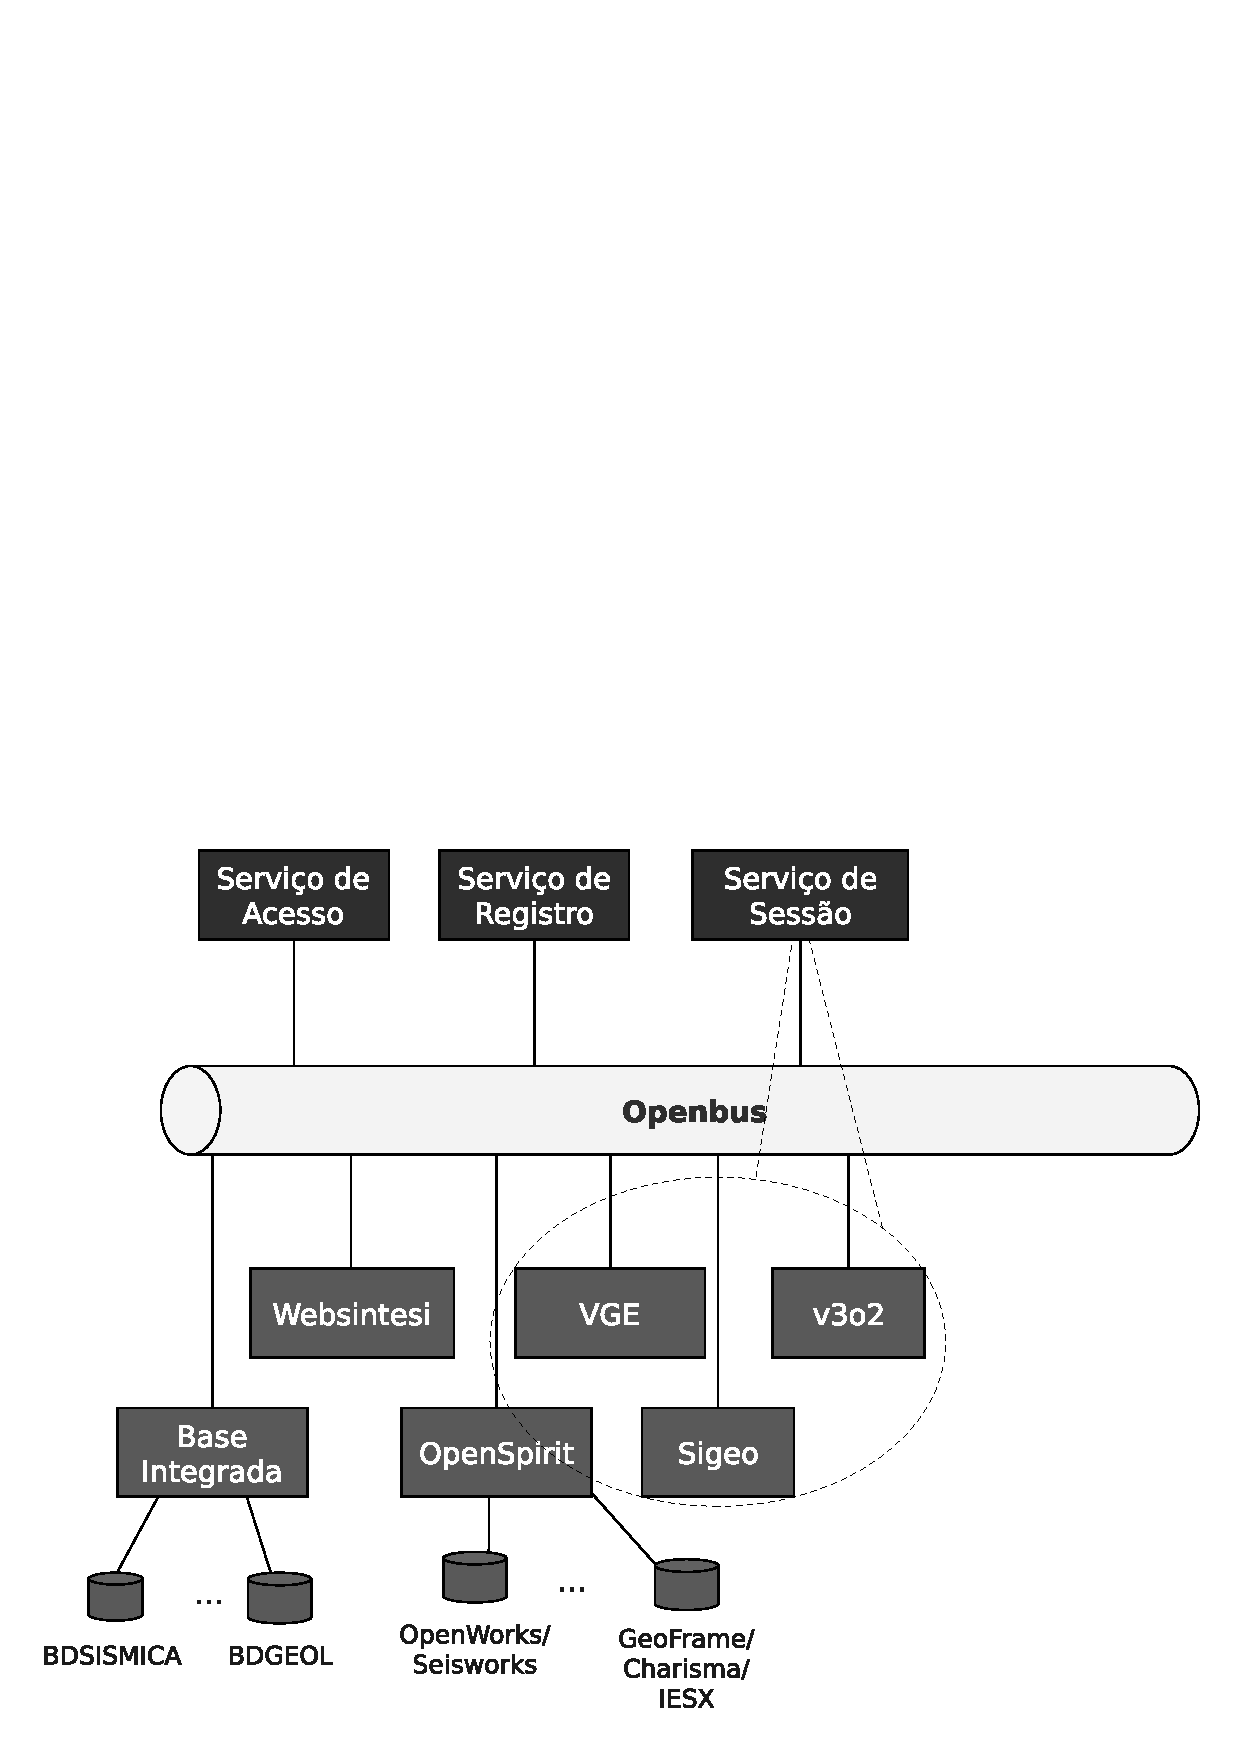
\includegraphics[width=14cm]{figs/arquitetura.pdf} %height=3in, 
\caption{Arquitetura do \openbus}
\label{fig:architecture}
\end{figure}

Qualquer aplica��o que queira fazer parte do barramento deve
implementar um componente para o \openbus. Atrav�s desse componente
� poss�vel acessar todos os servi�os existentes no barramento.
Para isso, o componente deve ser capaz de se conectar ao barramento e se
autenticar.
Atrav�s dos servi�os oferecidos pelo \openbus, o componente pode acessar
um servi�o previamente conhecido, ou pode consultar o servi�o de
localiza��o para descobrir qual componente oferece o servi�o que ele
deseja acessar.
Para oferecer um servi�o, uma aplica��o pode usar o mesmo componente ou
implementar outro. Tal componente deve ser capaz de publicar no
barramento a interface do servi�o que deseja oferecer.

%\subsection{Servi�os b�sicos}

Entre os servi�os b�sicos oferecidos pelo \openbus\/ podemos destacar os
servi�os de autentica��o, localiza��o, troca de mensagens e colabora��o.

\begin{itemize}
%%%%%%%%%%
\item Servi�o de autentica��o 
%%%%%%%%%%

Para fazer parte do barramento, um componente deve se autenticar a ele.
Existem tipicamente duas formas de autentica��o para um
componente. Uma onde o componente usa a credencial de um usu�rio e outra
onde o componente (ou aplica��o) possui uma credencial pr�pria.

Aplica��es como o VGE, onde o usu�rio fornece seu identificador e sua
senha, podem usar a pr�pria credencial do usu�rio para 
autenticar seus componentes no barramento.
J� as aplica��es que executam como um {\em daemon} podem utilizar uma
credencial pr�pria.

Como apenas um componente do barramento pode acessar servi�os de outro
componente e todos os componentes do barramento j� foram autenticados,
os componentes do barramento s�o considerados confi�veis.
Entretanto, cabe a cada servi�o verificar se um componente possui a
devida autoriza��o para acessar seus servi�os.

%%%%%%%%%%
\item Servi�o de localiza��o 
%%%%%%%%%%

O servi�o de localiza��o � baseado no servi�o de {\em trading} de 
CORBA. Este servi�o facilita a oferta e o descobrimento de inst�ncias de
servi�os de tipos espec�ficos.
Com este servi�o, componentes podem publicar suas caracter�sticas
e outros componentes podem encontrar os servi�os desejados
atrav�s das caracter�sticas publicadas.

Para publicar um servi�o, um componente prov� ao servi�o de localiza��o
uma descri��o de seu servi�o e a sua localiza��o.
Para encontrar um servi�o, um componente pergunta ao servi�o
de localiza��o se existe algum servi�o com determinadas caracter�sticas.
O servi�o de localiza��o procura entre as descri��es que possui e
responde com a localiza��o da interface do servi�o selecionado.
O componente que solicitou o servi�o pode ent�o acess�-lo.

%%%%%%%%%%
\item Servi�o de troca de mensagens
%%%%%%%%%%

O servi�o de troca de mensagens � baseado no servi�o de notifica��o de 
CORBA.
Atrav�s dele, as aplica��es podem comunicar-se livremente,
trocando mensagens diretas ou registrando interesse em receber 
mensagens quando algum even\-to ocorre na outra aplica��o.

Quando duas aplica��es est�o vendo o mesmo dado e uma delas o altera, 
atrav�s desse servi�o, ela pode enviar uma mensagem para a outra
aplica��o para que ela atualize a sua c�pia do dado.

%\begin{figure} [htb]
%\centering
%\includegraphics[width=8cm]{figs/eventos.pdf} %height=3in, 
%\caption{Troca de mensagens}
%\label{fig:datachange}
%\end{figure}

%%%%%%%%%%
\item Servi�o de colabora��o
%%%%%%%%%%

O servi�o de colabora��o usa o servi�o de troca de mensagens.
Atrav�s dele, um componente pode criar uma sess�o de
colabora��o e definir quem s�o os componentes participantes.
Inicialmente, cada componente � convidado pelo servi�o de colabora��o
a fazer parte desta sess�o.

Cada sess�o de colabora��o possui atributos espec�ficos e pode envolver
mais de um tipo de aplica��o de diferentes usu�rios.
Por exemplo, uma colabora��o entre diferentes inst�ncias 
do v3o2 pode ter atributos de c�mera, para que as diferentes inst�ncias
tenham a mesma vis�o do volume (Figura~\ref{fig:architecture}.)
Atrav�s de uma sess�o, os componentes envolvidos podem compartilhar
diferentes tipos de eventos, como por exemplo, eventos de intera��o
de usu�rio (sele��o e altera��o de dados, movimenta��o de cursor). Cada
componente pode gerar e receber esses eventos.

\end{itemize}



\section{Conclus�es}
\label{conclusoes}

Com a utiliza��o do OpenBus as dificuldades apontadas no fluxo de
trabalho das integra��es atuais ser�o eliminadas. Toda integra��o entre
aplica��es consistir� em conectar as aplica��es em quest�o ao ambiente
de execu��o OpenBus (AEOB). Com essa padroniza��o, ser� mais f�cil para
os desenvolvedores das aplica��es implementarem as integra��es exigidas
e, com isso, o n�mero de aplica��es integradas dever� aumentar.

A integra��o das aplica��es comerciais ser� bastante facilitada tamb�m,
pois o �nico trabalho de integra��o exigido ser� a cria��o de um driver
para comunica��o com o AEOB. Dado que uma aplica��o comercial est�
conectada ao AEOB, qualquer aplica��o Petrobras conectada ao AEOB poder�
obter os dados disponibilizados por essa aplica��o comercial. Como a
integra��o com uma aplica��o comercial ser� transparente, ser� poss�vel
remover aplica��es comerciais que deixem de ser interessantes sem a
necessidade de altera��o nas aplica��es Petrobras, desde que uma outra
aplica��o qualquer disponibilize o mesmo tipo de dado.

Com o aumento das integra��es, o usu�rio deixar� de lado o papel de
integrador e poder� focar na tarefa que deseja realizar, aumentando sua
produtividade.

Para um melhor aproveitamento do OpenBus, dever� ser implementada uma
extens�o para o dom�nio de Geologia e Geof�sica.



\end{document}
